\documentclass{beamer}
\usepackage[utf8]{inputenc}
\usepackage{hyperref}
\usepackage{listings}
\usepackage{subcaption}
\usepackage{amsmath}
\usepackage{mathtools}


\lstdefinestyle{saneCode}{
    belowcaptionskip=1\baselineskip,
    breaklines=true,
    frame=none,
    numbers=none,
    basicstyle=\tiny\ttfamily,
    % keywordstyle=\bfseries\color{green!40!black},
    commentstyle=\itshape\color{purple!40!black},
    % identifierstyle=\color{blue},
    backgroundcolor=\color{gray!10!white},
    keepspaces,
    upquote=true,
    showstringspaces=false,
}

\usetheme{Singapore}
\usecolortheme{default}

\title{Seeing the Unseen with Machine Learning}
\subtitle{A Physics-Informed Neural Network Approach to Inverse Problems}
\author[Thompson, Nameika]{
  Nameika, Michael \\
  \and
  Thompson, Jonathan
}

\institute[UCCS]{University of Colorado at Colorado Springs}

\date[UCCS 2023]
{May 08, 2023}

% \logo{\includegraphics[height=1cm]{overleaf-logo}}

\begin{document}
\beamertemplatenavigationsymbolsempty

% Title Page
\frame{\titlepage}

% Presentation Content
\begin{frame}
    \frametitle{The Problem}

    Given a physical system for which we have some experimental data, can we utilize machine learning to understand the
    physics of the system?
    \bigskip

    \begin{figure}
        \centering
        \begin{subfigure}[b]{0.45\textwidth}
            \centering
            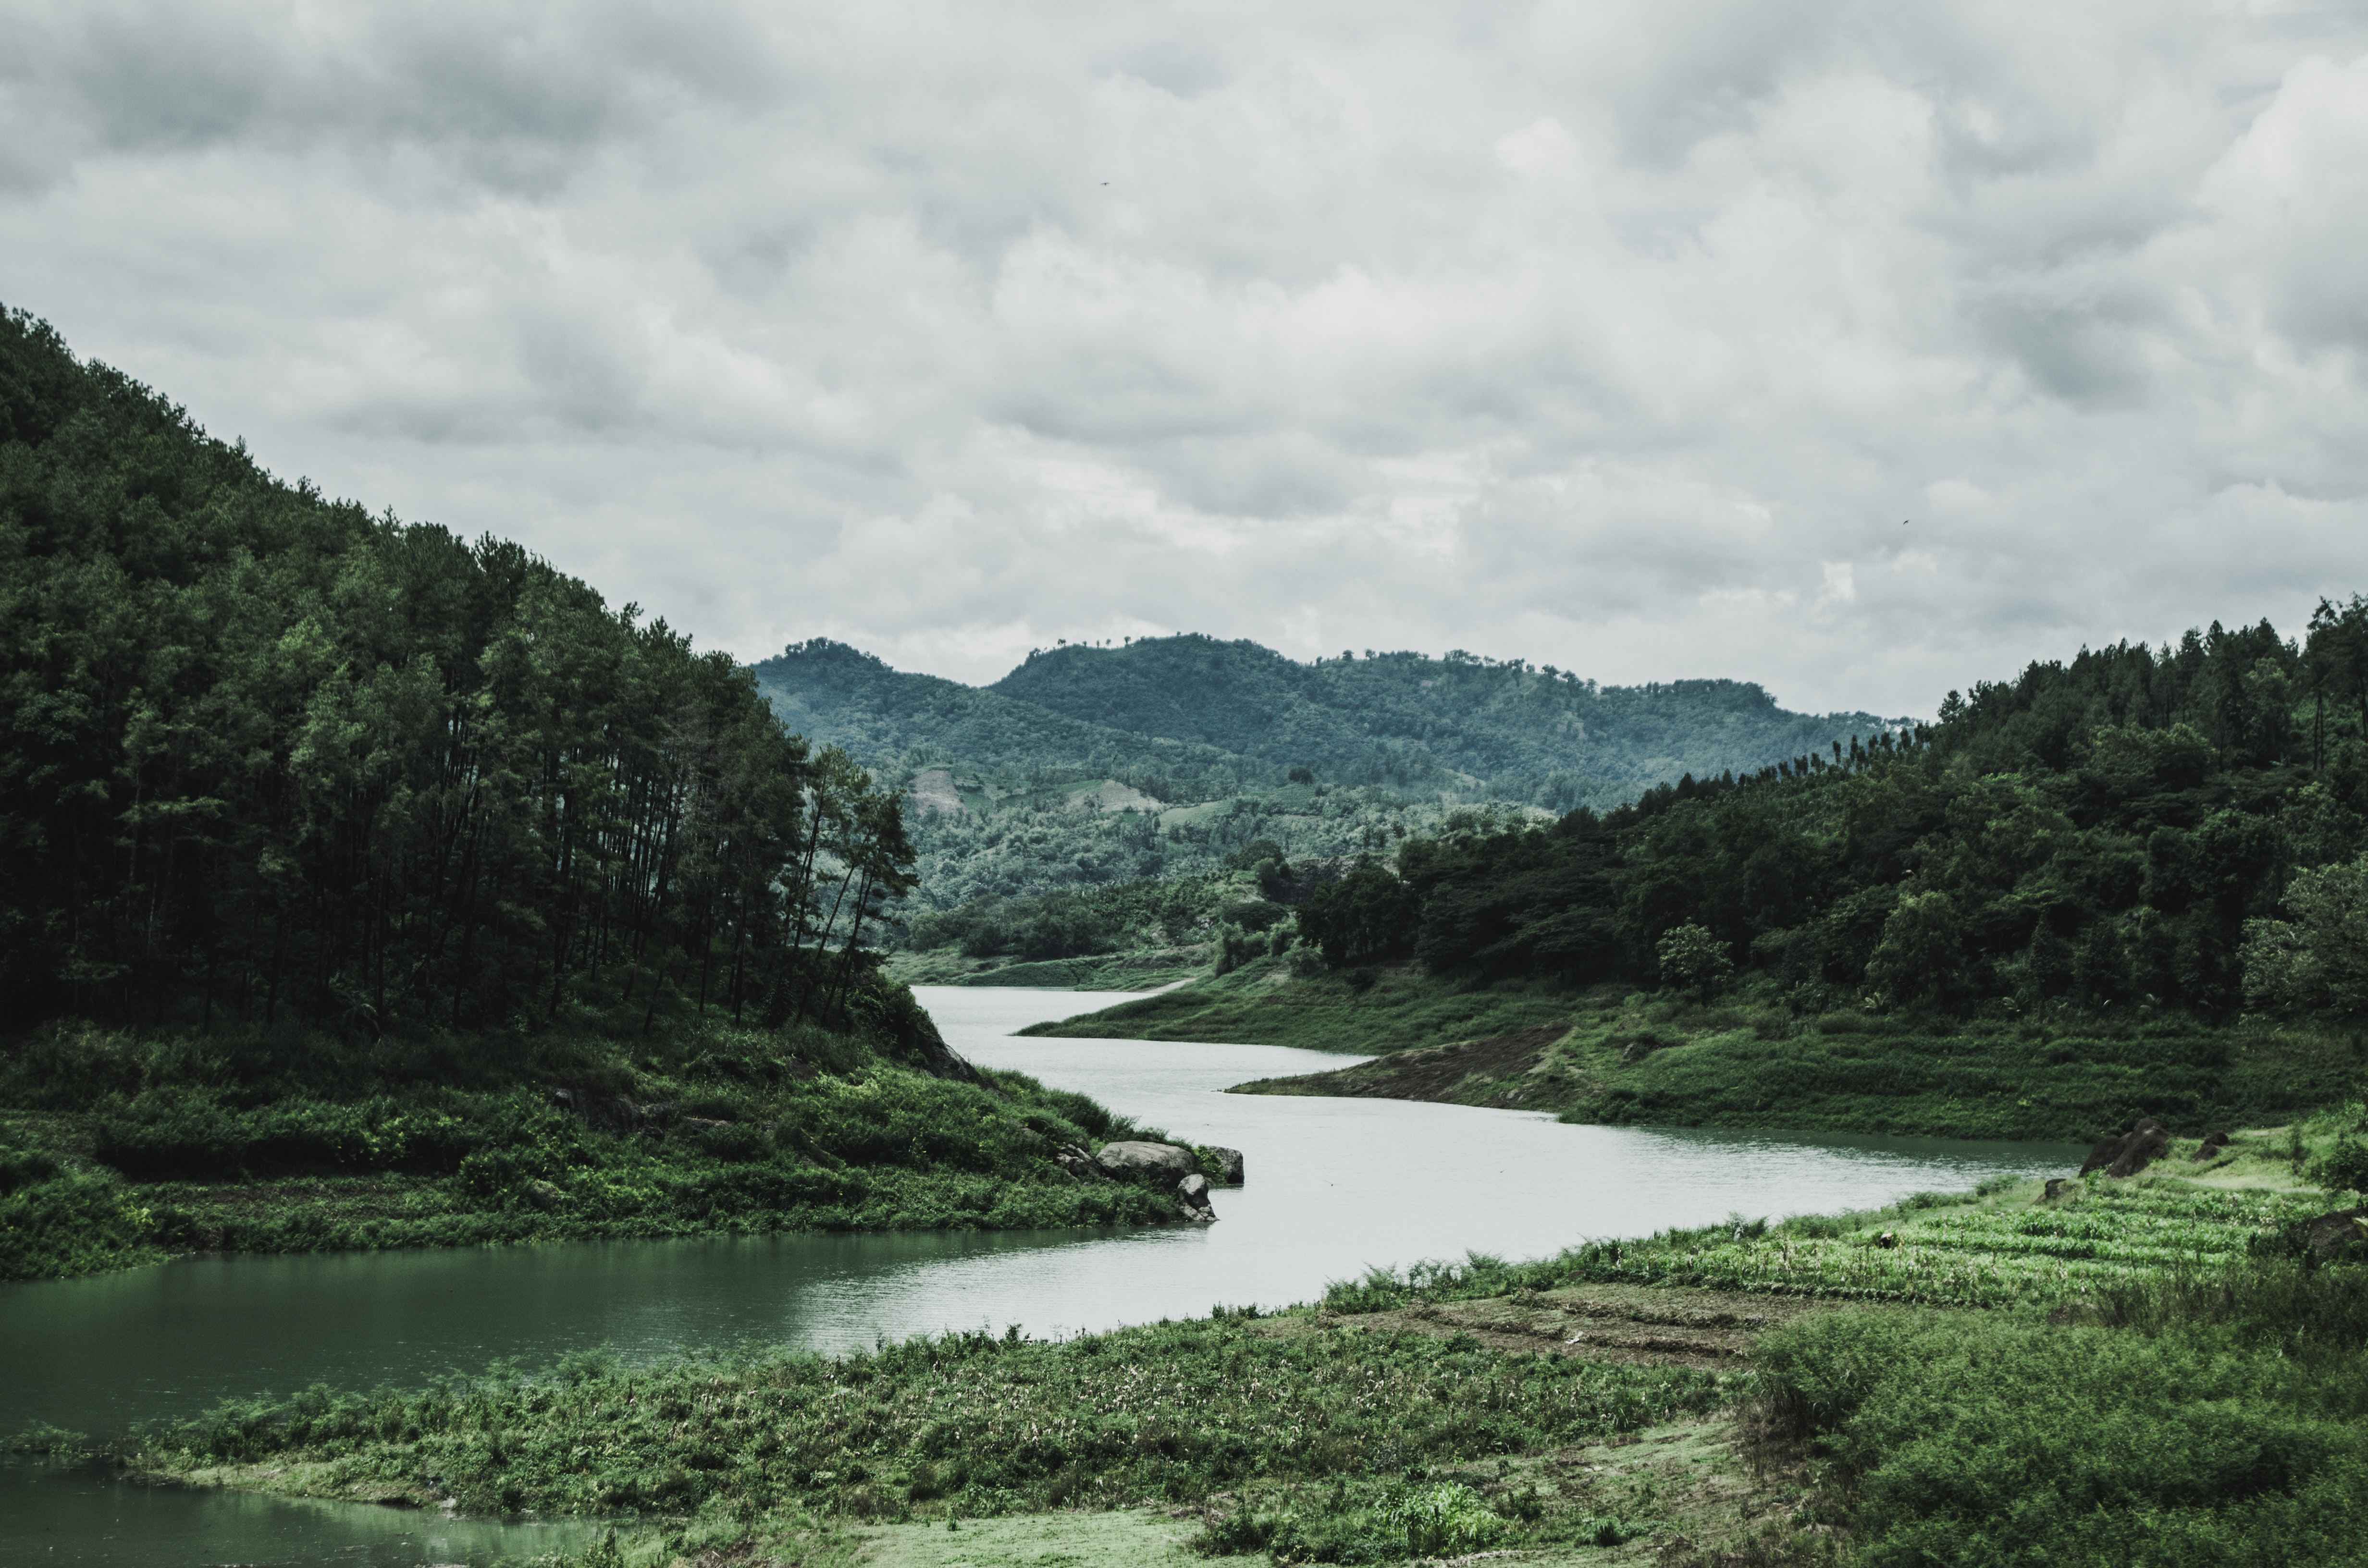
\includegraphics[width=\textwidth]{images/pexels-rido-alwarno-1034887.jpg}
            \caption{A river.}
            \label{fig:01_river}
        \end{subfigure}
        \hfill
        \begin{subfigure}[b]{0.45\textwidth}
            \centering
            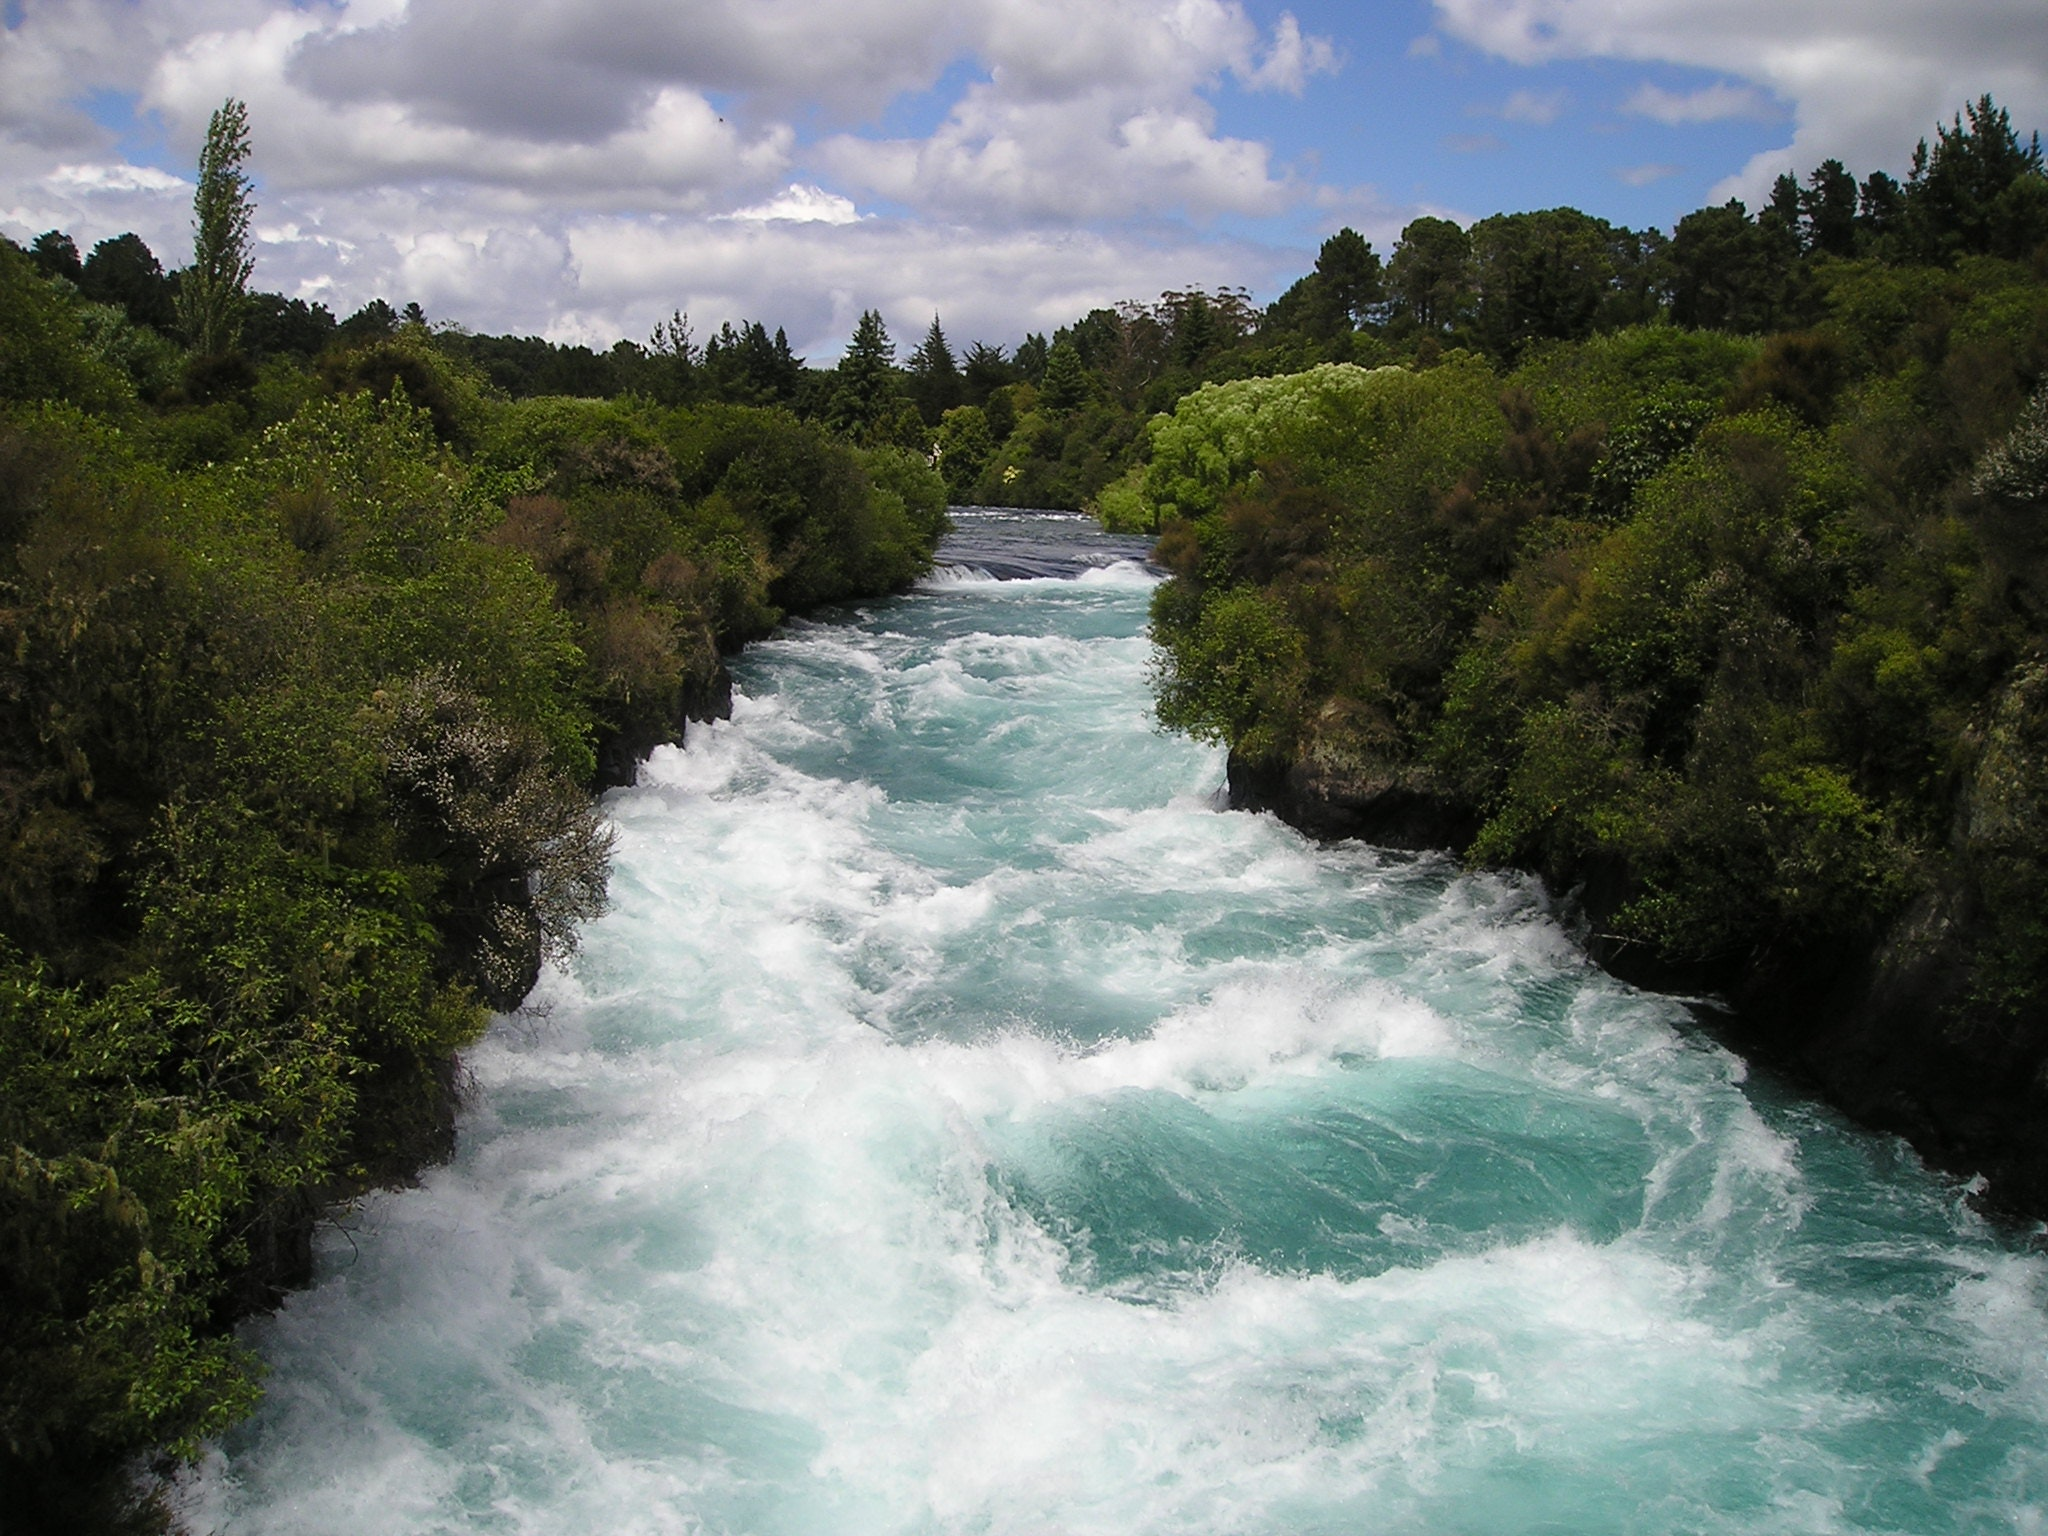
\includegraphics[width=\textwidth]{images/pexels-pixabay-2438.jpg}
            \caption{An angry river.}
            \label{fig:01_angry_river}
        \end{subfigure}
        \caption{Natural wave phenomena.}
        \label{fig:rivers}
    \end{figure}
\end{frame}
\begin{frame}
    \frametitle{Background}

    We explore this question in the context of the 1D Shallow-Water Equations (SWE).
    \bigskip

    \pause 
    The SWEs are a system of hyperbolic partial differential equations (PDE) which represent a simplified model of fluid
    flow.

    \bigskip
    \pause
    These equations are derived from the Navier-Stokes equations where the horizontal length scale is
    much greater than the vertical length scale (e.g., oceanic modeling, river flow, flood waves, etc.).
\end{frame}
\begin{frame}
    \frametitle{The Equations}

    \ \\
    \setlength{\belowcaptionskip}{-20pt}
    \begin{figure}
        \centering
        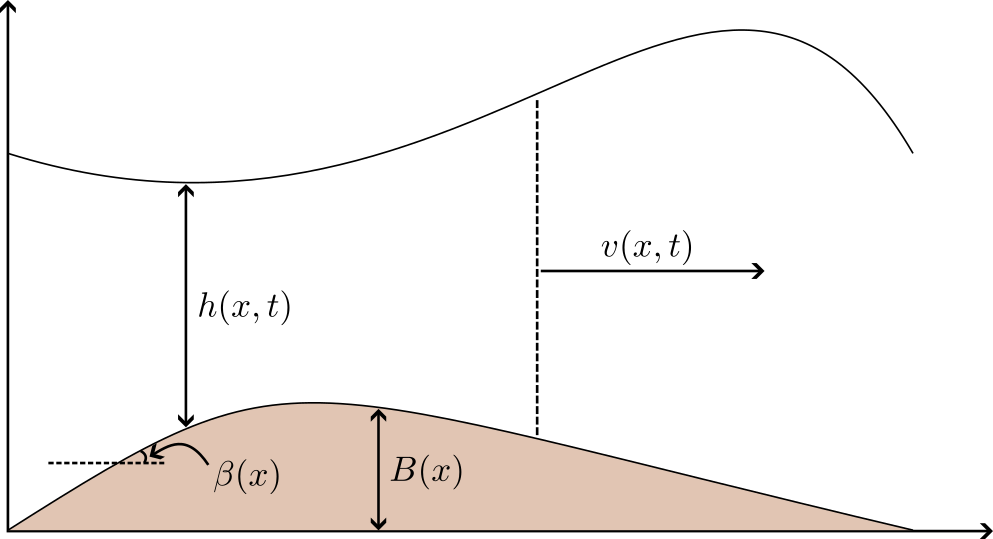
\includegraphics[width=0.7\textwidth]{images/swe_diagram.png}
        \caption{SWE Formulation. $\tan{\alpha} = B_x$}
        \label{fig:03_swe_diagram}
    \end{figure}

    \begin{align*}
           & h_t + (h v)_x = 0 & \text{(mass)} \\
           & (h v)_t + \left[ hv^2 + \frac{1}{2} g h^2 \cos{(\alpha)} \right]_x - g h \sin{(\alpha)} + C_f v^2 = 0 & \text{(momentum)}
    \end{align*}
\end{frame}
\begin{frame}
    \frametitle{Methodology: Approximation}

    Given some initial state (boundary conditions and initial conditions) of the system, we'd like to find out how
    $h(x, t)$, $v(x, t)$, and $\beta(x)$ evolve over space and, where applicable, time.

    \bigskip
    \pause
    Systems like this are rarely solveable analytically, so we utilize a numerical approach. 

    \bigskip
    \pause
    One such approach is to create an analytic approximation function $\mathcal{N}: \mathbb{R}^2 \to \mathbb{R}^3$ to the true solution so that:

    $$
    \mathcal{N}(x, t) = \begin{pmatrix*}
        \mathcal{N}_h \\
        \mathcal{N}_v \\
        \mathcal{N}_\beta 
    \end{pmatrix*} \approx \begin{pmatrix*}
        h \\
        v \\
        \beta
    \end{pmatrix*}.
    $$
\end{frame}
\begin{frame}
    \frametitle{Methodology: Residual}

    We are almost ready to frame this as an unconstrained optimization problem. To do so, we substitute our approximation 
    function into the SWE system. 

    \bigskip
    \pause

    Since we're only approximating the solution, we expect there to be some amount ``left over", which we call the 
    \textit{residual} and denote $R$. 
    
    \bigskip
    \pause

    The first equation in the system 
    
    $$
    h_t + (hv)_x = 0
    $$
    
    yields the residual term associated with conservation of mass:

    $$
    \left( \mathcal{N}_h \right)_t + \left( \mathcal{N}_h \mathcal{N}_v \right)_x = R_{mass}(x, t).
    $$

    \bigskip
    \pause

    The residual term associated with the momentum is similarly obtained from the second equation, which we denote 
    $R_{momentum}$.
\end{frame}
\begin{frame}
    \frametitle{Methodology: Optimization}

    We find the best approximation to the true solution by solving the non-linear unconstrained minimization problem:

    $$
    \min_{\mathcal{N}} {\lVert R_{mass} \rVert + \lVert R_{momentum} \rVert}.
    $$

    \bigskip
    \pause

    At this point, we have a well-defined optimization problem, but we still need to decide what our approximation 
    function $\mathcal{N}$ "looks like". 

    \bigskip
    \pause

    Ideally, we'd like a function which can modified to minimize the PDE residual via existing optimization algorithms.
\end{frame}
\begin{frame}
    \frametitle{Implementation}

    Neural networks fit the bill! What are they?

    \medskip
    \pause

    A (feedforward) neural network is an affine composition (e.g., $f(g(x)) = m g(x) + b$) of multivariate ``squashing''
    functions, such as the sigmoid or hyperbolic tangent functions. 
   
    \bigskip
    \pause More importantly, for particular choices of ``squashing" functions, neural networks are:
    \bigskip

    \begin{itemize}
        \setlength\itemsep{1.5em}
        \item Universal function approximators (for Borel-measurable functions over compact domains).
        \item Infinitely differentiable (analytic).
        \item Trainable via gradient descent (by modifying the coefficients $m$ and $b$ of the affine maps).
    \end{itemize}
\end{frame}
\begin{frame}
    \frametitle{Optimization Algorithms}

    Since neural networks have a \textit{lot} of parameters to train, we use stochastic gradient descent variations to 
    make the training process possible on modern hardware.

    \bigskip
    \pause

    In stochastic gradient descent, we use random subsets of the training data to compute the gradient of the residual
    in place of the entire set.

    \bigskip
    \pause

    \textbf{Adaptive Moment Estimation (Adam)}
    \ \\
    \bigskip

    [\textbf{TODO:} Describe Hessian approximation ]

    \pause
    \bigskip

    \textbf{Limited-Memory BFGS (L-BFGS)}
    \ \\
    \bigskip
    [\textbf{TODO:} Describe Hessian approximation ]
\end{frame}

\end{document}